%%%%%%%% ICML 2019 EXAMPLE LATEX SUBMISSION FILE %%%%%%%%%%%%%%%%%

\documentclass{article}

% Recommended, but optional, packages for figures and better typesetting:
\usepackage{microtype}
\usepackage{graphicx}
\usepackage{subfigure}
\usepackage{booktabs} % for professional tables
\usepackage{amsmath}
\usepackage{algorithm}
\usepackage{algorithmic}

% hyperref makes hyperlinks in the resulting PDF.
% If your build breaks (sometimes temporarily if a hyperlink spans a page)
% please comment out the following usepackage line and replace
% \usepackage{icml2019} with \usepackage[nohyperref]{icml2019} above.
\usepackage{hyperref}

% Custom imports
\usepackage{pifont}% http://ctan.org/pkg/pifont
\newcommand{\cmark}{\ding{51}}%
\newcommand{\xmark}{\ding{55}}%

% Attempt to make hyperref and algorithmic work together better:
\newcommand{\theHalgorithm}{\arabic{algorithm}}

\usepackage[usenames,dvipsnames]{xcolor}
\definecolor{shadecolor}{gray}{0.9}
\newcommand{\red}[1]{\textcolor{BrickRed}{#1}}
\newcommand{\orange}[1]{\textcolor{BurntOrange}{#1}}
\newcommand{\green}[1]{\textcolor{OliveGreen}{#1}}
\newcommand{\blue}[1]{\textcolor{MidnightBlue}{#1}}
\newcommand{\sky}[1]{\textcolor{SkyBlue}{#1}}
\newcommand{\gray}[1]{\textcolor{black!60}{#1}}

\newcommand{\ux}{{\mathbf{x}}}

% Use the following line for the initial blind version submitted for review:
% \usepackage{icml2019}

% If accepted, instead use the following line for the camera-ready submission:
\usepackage[accepted]{icml2019}

% Use to make suggestions
\newcommand{\disi}[1]{\textcolor{Red}{[#1]\textsubscript{Disi}}}
\newcommand{\styvers}[1]{\textcolor{Red}{[#1]\textsubscript{Mark}}}  % Sorry \mark is already defined
\newcommand{\padhraic}[1]{\textcolor{Red}{[#1]\textsubscript{Padhraic}}}
\newcommand{\robby}[1]{\textcolor{Red}{[#1]\textsubscript{Robby}}}

% Uncomment to disable suggestions for final draft
% \newcommand{\disi}[1]{}
% \newcommand{\mark}[1]{}
% \newcommand{\padhraic}[1]{}
% \newcommand{\robby}[1]{}

% The \icmltitle you define below is probably too long as a header.
% Therefore, a short form for the running title is supplied here:
%\icmltitlerunning{Submission and Formatting Instructions for ICML UDL Workshop 2019}
\icmltitlerunning{Bayesian Evaluation of Black-Box Classifiers}

\begin{document}

\twocolumn[
\icmltitle{Bayesian Evaluation of Black-Box Classifiers}

% It is OKAY to include author information, even for blind
% submissions: the style file will automatically remove it for you
% unless you've provided the [accepted] option to the icml2019
% package.

% List of affiliations: The first argument should be a (short)
% identifier you will use later to specify author affiliations
% Academic affiliations should list Department, University, City, Region, Country
% Industry affiliations should list Company, City, Region, Country

% You can specify symbols, otherwise they are numbered in order.
% Ideally, you should not use this facility. Affiliations will be numbered
% in order of appearance and this is the preferred way.
\icmlsetsymbol{equal}{*}

\begin{icmlauthorlist}
\icmlauthor{Disi Ji}{equal,cs}
\icmlauthor{Robert Logan}{equal,cs}
\icmlauthor{Padhraic Smyth}{cs}
\icmlauthor{Mark Steyvers}{cogsci}
\end{icmlauthorlist}

\icmlaffiliation{cs}{Department of Computer Science, University of California, Irvine, CA, USA}
\icmlaffiliation{cogsci}{Department of Cognitive Science, University of California, Irvine, CA, USA}

\icmlcorrespondingauthor{Disi Ji}{disij@uci.edu}

% You may provide any keywords that you
% find helpful for describing your paper; these are used to populate
% the "keywords" metadata in the PDF but will not be shown in the document
\icmlkeywords{Machine Learning, ICML}

\vskip 0.3in
]

% this must go after the closing bracket ] following \twocolumn[ ...

% This command actually creates the footnote in the first column
% listing the affiliations and the copyright notice.
% The command takes one argument, which is text to display at the start of the footnote.
% The \icmlEqualContribution command is standard text for equal contribution.
% Remove it (just {}) if you do not need this facility.

%\printAffiliationsAndNotice{}  % leave blank if no need to mention equal contribution
\printAffiliationsAndNotice{\icmlEqualContribution} % otherwise use the standard text.

\begin{abstract}
We propose a Bayesian framework for assessing performance characteristics of black-box predictors.

\end{abstract}

\section{Introduction}

%Machine learning prediction models are now being widely applied in areas such as consumer products, medicine, transportation, engineering, and more.
Machine learning prediction models, particularly deep learning models, are increasingly being deployed operationally across a wide range of application areas,  ranging from diagnosis of medical images \cite{kermany2018identifying}, to autonomous driving \cite{du2017fused}, to speech recognition \cite{hinton2012deep}.
Going forward there is increasing interest in pushing machine learning prediction models into everyday use, and software systems with embedded machine learning components are becoming commonplace.
%A vast number of embedded machine learning predictors will be deployed (and are already) in our mobile phones, in our vehicles, in our home energy management systems, in our hospitals, and so on.
Many of these machine learning predictors will in effect be black-boxes from the perspective of  the humans that are using them. For example, the predictive model may have been developed remotely by some commercial entity  and the predictor may be hosted as a  service in the cloud  \cite{sanyal2018tapas}.
%\robby{Too many parentheses. Maybe omit e.g. and just cite.}
In addition, for a variety of reasons (legal, cost, industry competition), the human user will typically have no access to the detailed workings of the model, how the model was trained, or what data the model was trained on.

In this context it is increasingly important to develop techniques that can provide accurate and robust assessments of the quality of a model's predictions.
However, it is well-known that the ``self-confidence" estimates provided by machine learning predictors can often be quite unreliable and miscalibrated \cite{zadrozny2002transforming,kull2017a}.
In particular, complex models such as deep networks with high-dimensional inputs $\ux$ (such as images or text) are often significantly overconfident \cite{gal2016dropout, guo2017calibration,lakshminarayanan2017simple,kuleshov2018accurate, keren2018calibrated}.

{\it Independent assessment} of accuracy and confidence for a predictor (rather than self-reported confidence or recalibration) will likely become increasingly important in the future.
By independent we mean assessment that is carried out independently from training procedures, perhaps by different individuals on different data, in a manner similar to the assessments of commercial products carried out by  regulatory agencies.
Reasons for independent assessment include the need for  building trust on the part of a human user of model predictions,  regulatory or legal reasons that may mandate independent assessment of models, or situations where the predictor is being used in an environment $p(\ux, y)$ which is different in an unknown way to the joint distribution in the environment that the model was trained on.
%$q(\ux, y)$ it was trained on.
%\robby{Omit $p$ and $q$ - don't need math symbols if they are undefined.}

In this workshop paper we present early results on the development of Bayesian approaches for independent assessment of the quality of black-box predictors, focusing on accuracy and calibration error for classification models.
We develop a number of concepts that underlie our proposed framework and illustrate the potential approach using image and text classification datasets.
We view our paper as preliminary work that should spur further discussion and interest among attendees of this workshop.


\section{Related Work}

While there is plenty of prior work in machine learning on calibration and recalibration methods for classification models, there is relatively little work on quantifying uncertainty in this context.
Some very recent work (of which we just became aware before submission of this paper) is that of \cite{vaicenavicius19a} who propose a general framework for evaluation of classification model calibration, including the use of bootstrap to obtain confidence intervals on the degree of miscalibration of a model, building on earlier work that also proposed the bootstrap in a calibration context \cite{brocker2007increasing}.
This paper could be viewed as the Bayesian alternative to the more frequentist perspective proposed in \cite{vaicenavicius19a}.
In addition, we go beyond just calibration measures and also statements related to classifier accuracy and assessing uncertainty about such statements from a Bayesian perspective.


\section{Framework}

Consider a classification problem with a feature space $\ux$ and a class label $y$ taking $K$ values, e.g., classifying image pixels $\ux$ into one of $K$ classes.
We have a prediction model $M$ that has already been trained on training data and that makes predictions $\hat{y}_M \in \{1, \ldots, K\}$ given a feature vector $\ux$.
The model can also produce numerical scores per class reflecting its confidence, typically in the form of a set of class probabilities $\hat{p}_M(y = k | \ux), k = 1,\ldots,K$.
These scores or probabilities in general need not be calibrated, i.e., they need not match the true probabilities $p(y=k | \ux)$.
The problem we focus on is Bayesian estimation of the performance of a model $M$ on data drawn from some distribution $p(\ux,y)$, a distribution that need not be the same as the distribution the model was trained on.
%or unnormalized $z_k(\ux)$ (unnormalized), $1 \le k \le K$---

We are interested in the situation where the model $M$ is a black-box where we can observe the inputs $\ux$ and the outputs $\hat{p}_M(y = k | \ux)$ but don't have any other information about the inner-workings of $M$ and the model $M$'s parameters are fixed.
%we are a ``consumer" of a prediction model $M$  and don't have any way to update it.
This is likely to be an increasingly common scenario as machine learning models are developed as a software service and deployed across many applications.
Note while our setup is Bayesian, it is different to the usual notion of Bayesian deep learning in the literature: we assume that the model's predictions are fixed and not changeable and we are only interested in assessment.
The predictions themselves can come from any black-box model (including Bayesian or non-Bayesian predictive models).


\section{Notation}

We will use $k^* = \arg \max_k \hat{p}_M(y = k | \ux)$ to denote the model $M$'s label prediction when the input is $\ux$.
We assume that the prediction model implements a deterministic mapping from the input space $\ux$ to $k^*$ (and for convenience that ties in the model's class scores $\hat{p}_M(y = k | \ux)$ are resolved deterministically).

The input space $\ux$ is partitioned by the model into $K$ decision regions $\mbox{R}_{k^*},  k^* = 1,\ldots,K$.
We can define conditional densities such as $p(\ux | k^*)$, which corresponds to the (normalized) density of $\ux$ conditioned on the fact that class $k^*$ is predicted by the model $M$, i.e., that $\ux \in \mbox{R}_k$.


We define $s_M(\ux) = \hat{p}_M(y = k^*| \ux) = \max_k \hat{p}_M(y = k | \ux)$ as the {\bf score} of the model as a function of $\ux$, i.e., the class probability that the model produces for its prediction $k^*$  given input $\ux$.
Under this notation, an expression such as $E_{p(\ux | k^*)}[s_M(\ux)]$ can be interpreted as the expected value of the model's score when it predicts class $k^*$, averaging over the $\ux$ values in decision region $\mbox{R}_{k^*}$, i.e.,
\[
    E_{p(\ux | k^*)}[s_M(\ux)] \ = \ \int s_M(\ux) p(\ux | k^*) d\ux
\]


\section{Local and Classwise Accuracy and Calibration Error}

The {\bf local accuracy} of a model can be defined locally at any point in $\ux$ as $A(\ux) = p(y = k^*| \ux)$ where $p(y | \ux)$ is the true uncertainty in $y$ conditioned on $\ux$.
%\robby{Not sure what $p(.. | \ux)$ means.}
The expected accuracy of the model over the whole $\ux$ space is $E_{p(\ux)}[p(y = k^*| \ux)] = \int p(y = k^*| \ux) p(\ux) d\ux$.
In machine learning this is typically estimated empirically on a test data set by drawing $S$ samples randomly from $p(\ux,y)$ and computing $\frac{1}{S} \sum_{i=1}^S I(y_i, k_i^*)$ where $k_i^*$ is the class predicted by the model given $\ux_i$.

We can also define the {\bf local calibration error} $CE(\ux)$ (see also \cite{vaicenavicius19a} of a prediction model as a function of $\ux$.
$CE(\ux)$ is the difference between the model's accuracy $A(\ux)$ and the model's own estimate of its accuracy at $\ux$, $p_M(y = k^*| \ux)$, i.e.,
\[
    CE(\ux) \ = \  \Delta\bigl(\ p_M(y = k^*| \ux), \  p(y =k^*| \ux) \  \bigr),
\]
where $\Delta(a,b)$ is some error measure such as absolute error. % $|a - b|$.

%To define the expected accuracy or calibration error per class we need to marginalize out $\ux$ over the decision region for class $k$, i.e., over $p(x|y_M^* = k)$:
%In this paper we explore other aggregate definition of calibration, in particular, accuracy per class.
We can marginalize over $\ux$ to compute the expected accuracy or calibration error per {\bf predicted class} $k^*$, expressed as conditional expectations $A_{k^*}  = E_{p(\ux|k^*)}[A(\ux)]$ and $CE_{k^*} = E_{p(\ux|k^*)}[ CE(\ux)]$, respectively, where the expectation is with respect to $\ux$ values in decision region $\mbox{R}_{k^*}$, i.e., conditioned on class $k^* $ being the predicted class\footnote{To get the accuracy or calibration error per {\bf true class} $k$ the expectations can be defined with respect to $p(\ux | y = k)$  rather than $p(\ux|k^*)$.}.

Performance measures such as calibration error and accuracy per predicted class can be useful in practice to a human user, for example in situations  when the model's predictions and probabilities are being used in a downstream application to make critical decisions with different costs (such as autonomous driving or medical diagnosis).
One example is the situation where the test environment $p(\ux,y)$ is significantly different to the environment the model was trained on---robust performance measures per class can provide a decision-maker with an important summary of what a model's actual performance will be for different predicted classes.

As an aside we note that calibration error is often expressed in the literature as a function of the model's score, in the form $CE(s_M)$, providing the basis for reliability diagrams with the score on the x-axis and the model's accuracy on the y-axis (e.g., \cite{guo2017calibration}).
The Bayesian framework we propose could be extended to Bayesian estimation of such functions, either bin-based or continuous (using for example Gaussian processes)---here we just focus on per class performance measures.
%\[
%CE(s_M) = E_{p(\ux|s_M)} [CE(\ux)] =   \int_{\ux} CE(\ux) p(\ux|s_M) d \ux
%\]
%=    \int_{\ux}  \max_k {p}_M(y = k | \ux) p(\ux |s_M) d \ux  $,
%and where $p(\ux |s_M)$ is defined along  isocontours of $\ux$ values in the input space that all produce the same score $s_M$.
%The expected calibration error (ECE, see \cite{naeini2015obtaining,guo2017calibration}) is in turn, $ECE = E_{p(\ux)}[\delta(p(y = k^*| \ux), s_M(\ux)] $.
%or with respect to scores $=E_{p(s_M)}[\delta(p(y = y_M^*| s_M(\ux)), s_M(\ux)] $.
%\int_{\ux}  \delta(p(y = y_M^*| \ux), s_M(\ux) p(\ux) d(\ux) $, or equivalently


\section{Bayesian Estimation of Accuracy and Calibration}\label{sec:bayesian}
Say we want to estimate the accuracy ${A}_{k^*}$ per predicted class $k^*$ from data. To estimate the integral empirically, we can sample $\ux,y$ pairs from the conditional distribution $p(x,y | k^*)$.
A standard approach in evaluation of classifier models would be to treat ${A}_{k^*}$ as an unknown Bernoulli parameter with ``draws" $I(y_i, k^*) \in \{0,1\}$ and compute a frequency-based (maximum likelihood) estimate
%\begin{equation}
\[
\hat{A}_{k^*} \ = \  \frac{1}{S} \sum_{i=1}^S A(\ux_i)
 \ = \ \frac{1}{S} \sum_{i=1}^S I(y_i, k^*), \ \ \ \ 1 \le k^* \le K
\]
%\end{equation}
where $k^*$ is the model's prediction for each of the $\ux_i$'s by definition.
However, given a finite amount of data for evaluation, and in situations where $K$ may be large, is natural to consider Bayesian estimation in this context, allowing for  uncertainty our inferences about quantities such as ${A}_{k^*}$.
In particular, we can put a Beta prior $Beta(\alpha, \beta)$ on ${A}_{k^*}$, model the draws $I(y_i, k^*)$ with a binomial likelihood, and produce Beta posteriors for each ${A}_{k^*}, k^* = 1,\ldots,K$

For calibration error, Bayesian estimation is a little more complex.
The frequency-based estimate of expected calibration error per class is
\begin{align*}
\hat{CE}_{k^*} & \ = \  \frac{1}{S} \sum_{i=1}^S CE(\ux_i), \ \  \ \ \ \ 1 \le k^* \le K \\
 &  \ = \  \frac{1}{S} \sum_{i=1}^S \Delta\bigl(p_M(y = k^*| \ux), \  p(y =k^*| \ux)  \bigr)
\end{align*}
The calibration error $\hat{CE}_{k^*}$ is bounded between 0 and 1 so it is natural to think of a Beta prior for $CE$ as we did for accuracy.
However, here we don't have binary draws (as we had with the indicator function for accuracy) but instead have a real-valued (bounded) quantity $\Delta(  )$ making Bayesian analysis less straightforward.
In this paper, for simplicity, we focus just on the {\bf calibration bias}  per class, where  $\Delta( ) = p_M(y = k^*| \ux) - p(y =k^*| \ux)$, in which case
$CE_{k^*} = %E_{p(\ux|k^*)}[ p_M(y = k^*| \ux) - A(\ux) ] =
E_{p(\ux|k^*)}[ p_M(y = k^*| \ux)] \ - \  {A}_{k^*} $.
\robby{Notsure what $\Delta(  )$ means.}
We will make the assumption that the uncertainty in estimating $CE_{k^*}$ will be dominated by the second term, ${A}_{k^*}$ since it requires labeled examples, whereas the first term (the average score for the model when class $k^*$ is predicted) can be estimated from unlabeled examples alone and thus, one can drive uncertainty about this term to zero with enough unlabeled data. Thus, for the case of Bayesian estimation of calibration bias, we will assume that the problem can be reduced to that of Bayesian estimation of accuracy.





\section{Illustrative Results}


\subsection{Experimental Setup}

\paragraph{Data}
We use the framework presented in the previous section to evaluate the performance of modern neural classifiers on the following datasets:
    CIFAR-100~\cite{krizhevsky2009learning},
    SVHN~\cite{netzer2011reading} and
    MHD~\cite{tai_seale2016mhd}.
CIFAR-100 and SVHN are standard benchmarks for deep model assessment ~\cite{guo2017calibration, hendrycks2019benchmarking}.
MHD was chosen since the label distribution is heavily skewed (the most common label applies to $30\%$ of instances whereas the least common label is observed $<1\%$ of the time), a property which helps illustrate the utility of Bayesian approaches to model evaluation.

\begin{table}[t]
    \centering
    \begin{tabular}{rcccc}
        \toprule
                        & Mode  & Size  & Classes   & Balanced  \\
        \midrule
             CIFAR-100  & Image & 60K   & 100       & \cmark    \\
             SVHN       & Image & 600K  & 10        & \cmark    \\
             PCORI      & Text  & 122K  & 27        & \xmark    \\
        \bottomrule
    \end{tabular}
    \caption{Dataset statistics.}
    \label{tab:datasets}
\end{table}

\paragraph{Models}
The model $M$ that we use for image classification tasks is a deep residual neural network (ResNet)~\cite{he2016deep} with 110 layers and 1.7 million parameters.
% This is the same model as used by \cite{guo2017calibration}.
For dialogue classification, we use a heirarchical recurrent neural network with gated recurrent units\robby{insert smodel details}.

%and Tiny ImageNet \cite{yao2015tiny, tinyimagenet}.
%We expect to have results for additional datasets available to report on by the time of the workshop.

%The classes are organized in a 2-level semantic hierarchy with 20 superclasses, each with 5 classes.  W
%The Tiny ImageNet dataset has 200 classes, each class with about 500 to 600 64 x 64 pixel images with known labels. The classes for this dataset do not have a predefined semantic hierarchy, but it will be straightforward to construct a 2-level hierarchy. State-of-the-art machine learning accuracy on CIFAR is around 85\% and on Tiny ImageNet is around 80\%, and accuracy varies considerably across the classes in each dataset.

\subsection{Classification Accuracy per Class}\label{sec:accuracy-experiment}

For illustration, we apply the beta-binomial model discussed in Section~\ref{sec:bayesian} to measure classwise accuracies for ResNet-110 predictions on CIFAR100.
Mean posterior estimates and 95\% credible intervals for the ten most and least accurate classes are plotted in Figure~\ref{fig:cifar100_acc}.
By examining which credible intervals overlap one another, we can see that it is uncertain which class is truly most accurate, whereas it is very certain that model performance is much better on the top ten classes than it is on the bottom ten.

\begin{figure}[t]
    \centering
    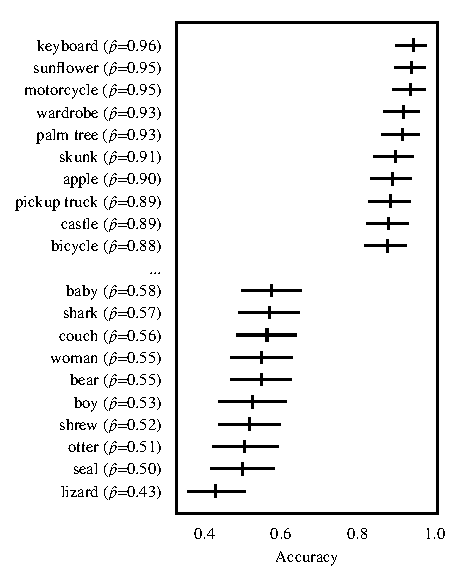
\includegraphics{figures/cifar100_accuracy.pdf}
    \caption{
        Mean posterior estimate and 95\% confidence intervals for the classwise accuracy of Resnet-110 predictions on CIFAR-100.
        Empirical accuracy estimates are listed next to the class labels.
        Overlapping bars indicate uncertainty about which class is the most/least accurate among classes in the top/bottom cohorts, however it almost certain that classes in the top cohort rank higher than classes in the bottom cohort.
    }
    \label{fig:cifar100_acc}
\end{figure}

An additional benefit of the Bayesian framework is that Monte Carlo sampling can be used to infer other statistics of interest from posterior distribution of calibration measures.
To provide a simple example, we use the classwise accuracy posteriors from the previous experiment to infer a probability distribution over accuracy rankings (e.g. Monte Carlo ranking~\cite{marshall1998league}).
A single ranking sample is obtained by drawing accuracy estimates $\tilde{A}_{k^*}$ from the posteriors for each class, and then ranking them.
95\% credible intervals for the ranks of the ten most and least accurate classes are plotted in Figure~\ref{fig:cifar100_rank}.
Similar to our previous result, we see that at the 95\% level we are uncertain about which class is the most/least accurate among classes in the top/bottom cohorts, but certain that classes in the top cohort rank higher than classes in the bottom cohort.

\begin{figure}[t]
    \centering
    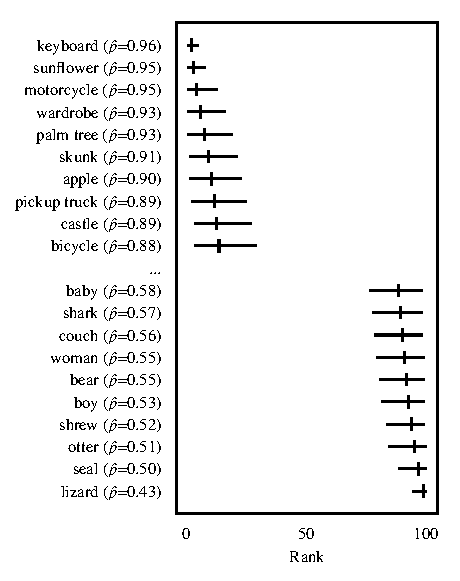
\includegraphics{figures/cifar100_rank.pdf}
    \caption{
        Approximate mean posterior estimate and 95\% confidence intervals for the rank of the most and least accurate classes predicted by Resnet-110 on CIFAR-100.
        Rank distributions estimated using 10K Monte Carlo samples.
    }
    \label{fig:cifar100_rank}
\end{figure}

% Make some qualitative statements, e.g., show examples (most accurate, least accurate). Could perhaps provide some statements based on 95\% credibility intervals, e.g., for the least accurate and most accurate class.

% Describe how we use use Monte Carlo ranking \cite{marshall1998league} based on draws from our Beta densities  to show the estimated ranks. Make some statements based on the figure, e.g., that we are 95\% confident that classes X, Y, and Z are in the top 10\% of the classes the model is most accurate for when predicting these classes, and likewise we are 95\% confidence that classes A, B, and C are among the 10\% least accurate.

% Perhaps comment generally that since we only have 100 data points per class that there are a large number of classes where we can't even say with any confidence whether they are among the top or bottom 50\% of classes in terms of rank.


\subsection{Calibration Bias per Class}

Similar analysis can be conducted to assess calibration bias.
Following the same setup as in Section~\ref{sec:accuracy-experiment} we obtain 95\% credible intervals for the calibration bias of
Figure~\ref{fig:cifar_bias} for example).




% \begin{figure}[h]
%  \centering
%    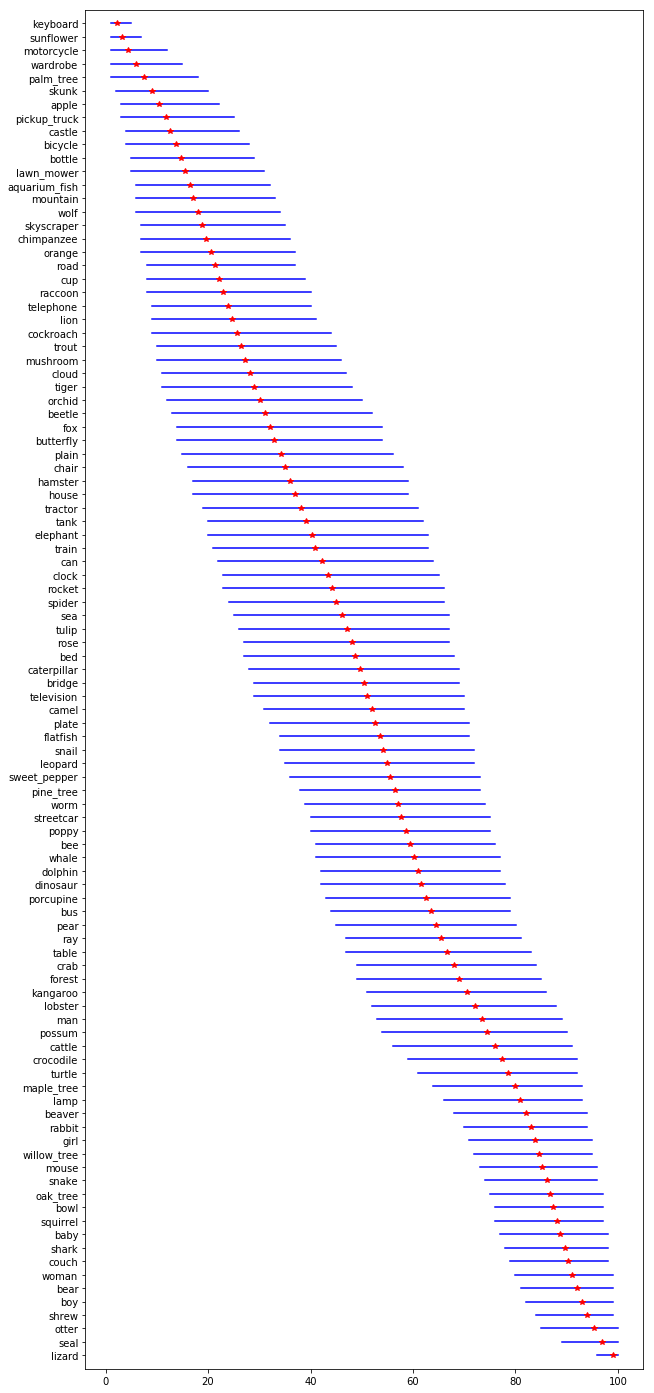
\includegraphics[width=0.4\textwidth]{figures/ranking_calibration_bias_CIFAR.png}
% \caption{MCMC-based ranking of calibration bias across predicted classes (where 1 corresponds to the class with the lowest calibration bias.}
% \label{fig:ranking_bias}
% \end{figure}

\subsection{Active Learning to Find Extreme Classes}

Thus far we have assumed access to a pool of labeled examples that can be used for model assessment.
This assumption is likely unrealistic in many real world scenarios.
Obtaining ground truth labels can be costly, this is one of the main motivations for using black-box models.
Accordingly, it is desirable for model assessment to be as data efficient as possible.

In this section, we demonstrate how the Bayesian framework we've presented can be paired with active learning techniques to design strategies that select data to be labeled, so that model assessment can be quickly performed.
Concretely, we focus on the task of finding the class with the worst classwise accuracy.
To achieve this we use a Thompson sampling~\cite{TODO} based approach (described in detail in Algorithm~\ref{alg:thompson}).

Results for 1k independent runs of this algorithm on CIFAR-100 are given in Figure~\ref{TODO}.
The x-axis is the number of queries made to the oracle.
The y-axis shows the fraction of runs where the correct class was identified as the class with the lowest expected accuracy.
As a baseline we also include results for when data points are selected at random.
This plot shows that the Thompson sampling based approach converges with much fewer queries.


\begin{algorithm}[tb]
   \caption{Thompson Sampling}
   \label{alg:thompson}
\begin{algorithmic}
	\STATE {\bfseries Input:} prior hyperparameters $\alpha$, $\beta$
	\STATE initialize $n_{k,0}=n_{k,1}=0$ for $k=1$ {\bfseries to} $K$
	\REPEAT
	\FOR{$k=1$ {\bfseries to} $K$}
        \STATE $\hat{A}_{k} \sim \text{Beta}(\alpha + n_{k,0}, \beta + n_{k,1})$
	\ENDFOR
	\STATE $k^{*} = \arg \min_k \hat{A}_{1:K}$
    \STATE select data point $(x, \hat{y}=k^{*})$
    \STATE query oracle for true label $y$
	\IF {$y = k^*$}
        \STATE $n_{k,0} \leftarrow n_{k,0} + 1$
	\ELSE
        \STATE $n_{k,1} \leftarrow n_{k,1} + 1$
    \ENDIF
	\UNTIL{all data labeled}
\end{algorithmic}
\end{algorithm}



\subsection{Other Possible Experiments}
\begin{itemize}
   \item CIFAR experiments with adversarial conditions, e.g., when the class distribution/accuracy/calibration changes significantly for 1 or more classes in the test data
   \item Extensions to handle absolute or squared calibration error
    \item Experiments with 1 or more additional data sets
    \item Experiments with another model (e.g. a simpler model) on the CIFAR data set, using Bayesian estimation to compare model accuracy (e.g., across classes).
    \item Inferences about the CIFAR confusion matrix
\end{itemize}
\section{Conclusions}

\newpage
\phantom{p}
\newpage
\bibliography{calibration}
\bibliographystyle{icml2019}


\newpage
\phantom{p}
\newpage


\section*{(Possible) Supplemental Materials}

\subsection*{Example: Bayesian Assessment of Calibration Error}

{\bf These earlier figures from Disi are included in case we want to show how Bayesian estimation can be applied to reliability diagrams, or at least to the binned versions. Perhaps put this in a supplement and contrast the inferences that one could make give 100 data points versus 10000 points}

Figure \ref{fig:betacalibration} shows a simple illustrative example of a Beta-Bernoulli model for Bayesian assessment of binned calibration values $\theta_c$ for the same SVHN deep learning model described earlier in Figure \ref{fig:misclassified}.
%In this particular example the assessor started with a weak prior that assumed the predictor is well-calibrated.
The third plot with $n=10000$ can effectively be treated as ground-truth: it shows that the predictor is significantly miscalibrated, producing class probability estimates that are higher than the corresponding empirical accuracy, i.e., it is overconfident.

\begin{figure}[h]
 \centering
  \subfigure{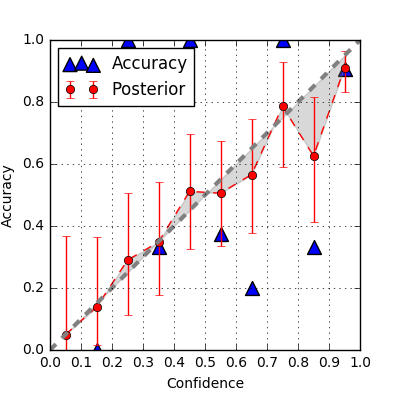
\includegraphics[width=0.3\textwidth]{figures/reliability_plot_100.png} } %\caption{$n=100$}}  %\label{fig:exph}}
  \subfigure{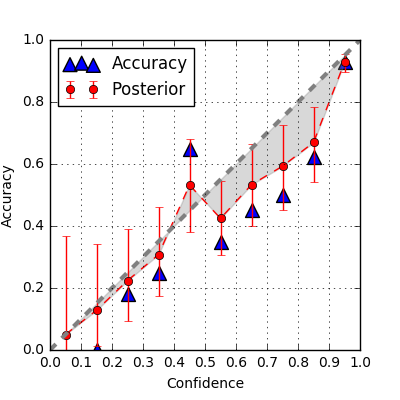
\includegraphics[width=0.3\textwidth]{figures/reliability_plot_500.png}} %\caption{$n=100$}}  %\label{fig:exgr}}
  \subfigure{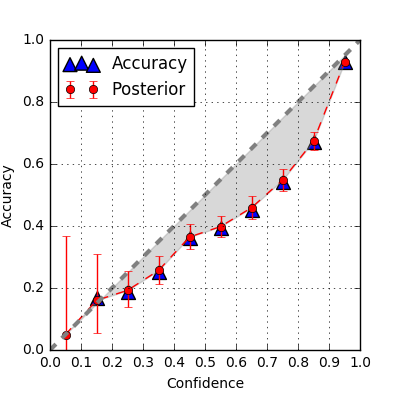
\includegraphics[width=0.3\textwidth]{figures/reliability_plot_10000.png}} %\caption{$n=100$}} %\label{fig:exgr}}

\caption{Bayesian assessment of calibration bins, for a deep neural network trained on the SVHN data, with different numbers of examples available to the assessor: $n=100$ (left), $n=500$ (center), $n=10000$ (right). The $x$-axis (Confidence) corresponds to bins for the estimated class probability provided by the deep network for the predicted class. The blue triangles on the $y$-axis are the empirically estimated accuracies per bin, given $n$ examples across all bins. The red dot and error bars on the $y$-axis correspond to the posterior belief of the assessor, namely the Bayesian posterior mean and 95\% credible intervals. The gray shaded area indicates the estimate (by the assessor) of the overall expected calibration error (ECE).}
\label{fig:betacalibration}
\end{figure}

%% CIFAR-100 RANKING PLOTS %%
\begin{figure}[t]
    \centering
    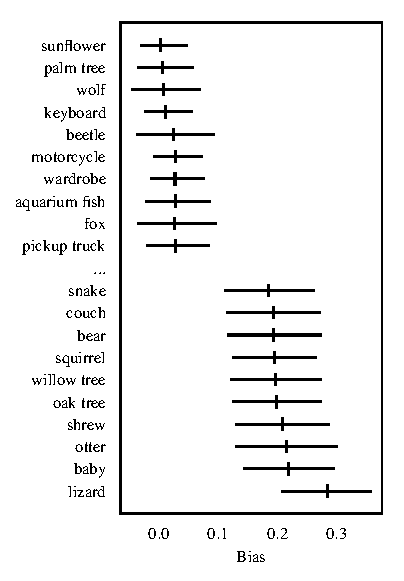
\includegraphics{figures/cifar100_bias.pdf}
    \caption{
        Mean posterior estimate and 95\% confidence intervals for the classwise calibration bias of Resnet-110 on CIFAR-100.
        Overlapping bars indicate uncertainty about which class is the most/least biased among classes in the top/bottom, however it almost certain that classes in the top cohort rank higher than classes in the bottom cohort.
    }
    \label{fig:cifar_bias}
\end{figure}

\begin{figure}[t]
    \centering
    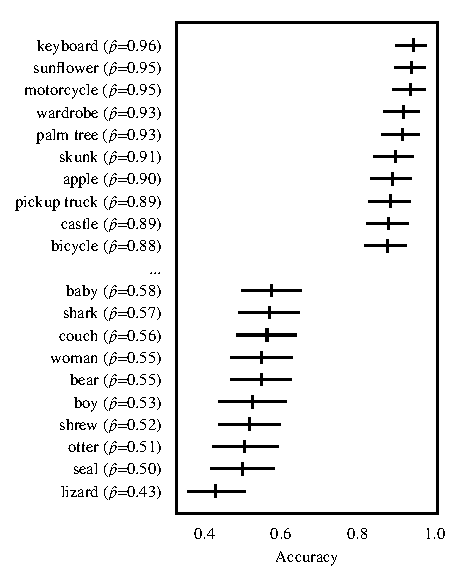
\includegraphics{figures/cifar100_accuracy.pdf}
    \caption{
        Mean posterior estimate and 95\% confidence intervals for the classwise accuracy of predictions by Resnet-110 on CIFAR-100.
        Overlapping bars indicate uncertainty about which class is the most/least accurate among classes in the top/bottom, however it almost certain that classes in the top cohort rank higher than classes in the bottom cohort.
    }
    \label{fig:cifar100_acc}
\end{figure}

\begin{figure}[t]
    \centering
    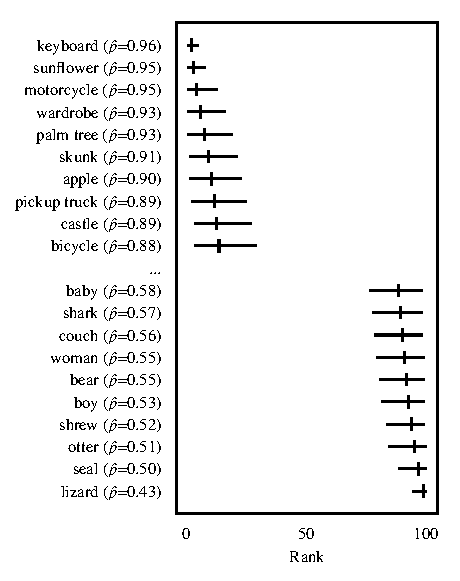
\includegraphics{figures/cifar100_rank.pdf}
    \caption{
        Mean posterior estimate and 95\% confidence intervals for the rank of the most and least accurate classes predicted by Resnet-110 on CIFAR-100.
        Overlapping bars indicate uncertainty about which class is the most/least accurate among classes in the top/bottom, however it almost certain that classes in the top cohort rank higher than classes in the bottom cohort.
    }
    \label{fig:cifar100_rank}
\end{figure}

%% SVHN RANKING PLOTS %%
\begin{figure}[t]
    \centering
    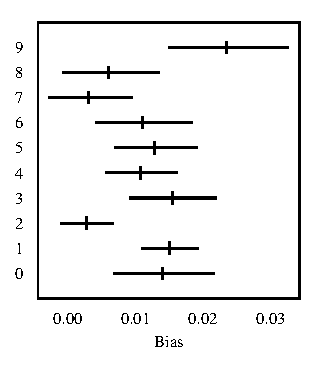
\includegraphics{figures/svhn_bias.pdf}
    \caption{
        Mean posterior estimate and 95\% confidence intervals for the classwise calibration bias of Resnet-110 on SVHN.
    }
    \label{fig:svhn_bias}
\end{figure}

\begin{figure}[t]
    \centering
    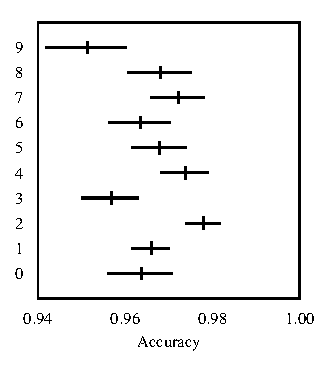
\includegraphics{figures/svhn_accuracy.pdf}
    \caption{
        Mean posterior estimate and 95\% confidence intervals for the classwise accuracy of predictions by Resnet-110 on SVHN.
    }
    \label{fig:svhn_acc}
\end{figure}

\begin{figure}[t]
    \centering
    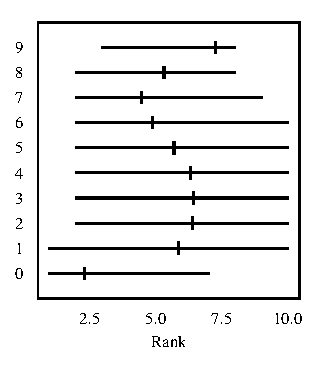
\includegraphics{figures/svhn_rank.pdf}
    \caption{
        Mean posterior estimate and 95\% confidence intervals for the rank of the most and least accurate classes predicted by Resnet-110 on SVHN.
    }
    \label{fig:svhn_rank}
\end{figure}

%% MHD RANKING PLOTS %%
\begin{figure}[t]
    \centering
    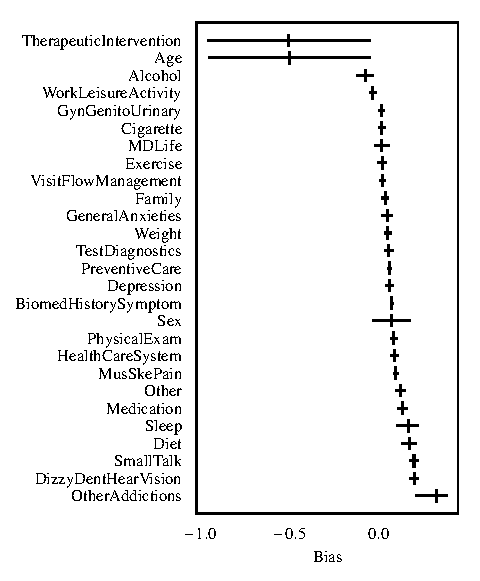
\includegraphics{figures/mhd_bias.pdf}
    \caption{
        Mean posterior estimate and 95\% confidence intervals for the classwise calibration bias of a hierarchical RNN on MHD.
        Unbalanced data results in a large amount of uncertainty for uncommon classes. % An 'Un'derstatement
    }
    \label{fig:mhd_bias}
\end{figure}

\begin{figure}[t]
    \centering
    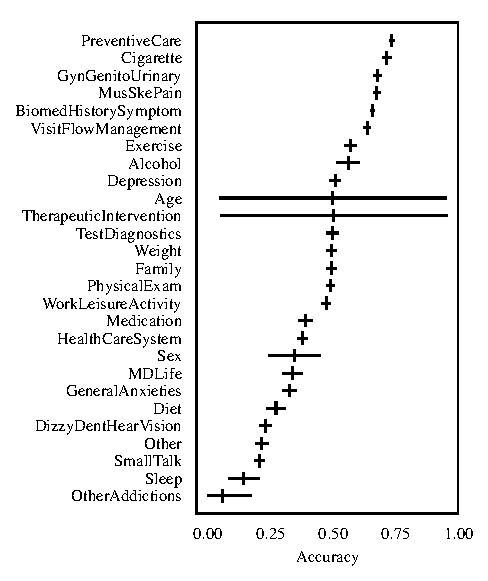
\includegraphics{figures/mhd_accuracy.pdf}
    \caption{
        Mean posterior estimate and 95\% confidence intervals for the classwise accuracy of a hierarchical RNN on MHD.
        Unbalanced data results in a large amount of uncertainty for uncommon classes.
    }
    \label{fig:mhd_acc}
\end{figure}

\begin{figure}[t]
    \centering
    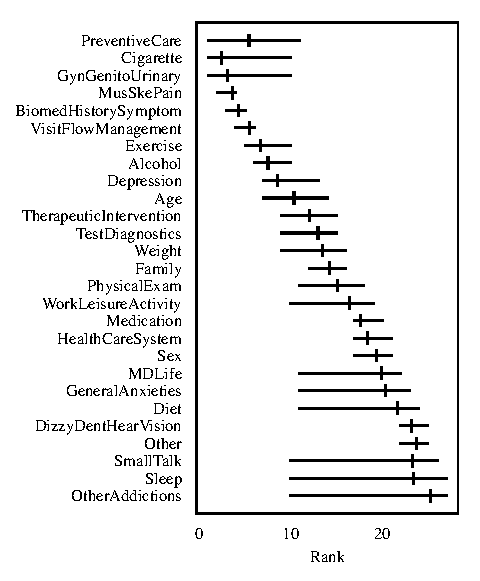
\includegraphics{figures/mhd_rank.pdf}
    \caption{
        Mean posterior estimate and 95\% confidence intervals for the rank of the most and least accurate classes predicted by a hierarchical RNN on MHD.
        }
    \label{fig:mhd_rank}
\end{figure}

 %To illustrate this point, Figure \ref{fig:misclassified} shows an example of misclassified test examples for a predictor trained to classify images into one of 100 classes (the SVHN collection\cite{krizhevsky2009learning}). The images shown in the figure are examples of images where the network is highly confident (class-conditional probabilities above 0.9 from the model) but where the predictions are incorrect.


\end{document}